\chapter{The Limited Proteolysis module}
\label{chap:limprot}

The Limited Proteolysis module is designed to post-process the results from an enzymatic digestion performed in two steps. The first step is assumed to be a limited proteolysis in which a large protein is split in smaller fragments. The fragments are then separated using a SDS-PAGE electrophoresis. Finally, selected bands from the gel are submitted to a full enzymatic digestion and the generated peptides are analyzed using mass spectrometry.

The main objective of the module is to identify the protein fragments generated in the initial limited proteolysis from the peptides found in the MS analyzed gel spots. This is achieved by performing an equivalence test\cite{Limentani2005} between the peptides in the selected gel spots and a control spot containing the full length target protein. In this way, peptides leaked from one gel spot to another can be eliminated. Several replicates of the experiment are expected.

\section{Definitions}
\label{sec:limprotDefinitions}

Before explaining in detail the interface of the module and how does the module works, lets make clear the meaning of some terms that will be used in the following paragraphs.

\phantomsection
\begin{itemize}
	\item \textit{Recombinant protein}: actual amino acid sequence used in the mass spectrometry experiments. It may be identical to the native sequence of the Target protein under study or not.
	\item \textit{Native protein}: full amino acid sequence expressed in wild type cells.
	\item \textit{Detected peptide}: any peptide detected in any of the mass spectrometry experiments including the control experiments.
	\item \textit{Relevant peptide}: a detected peptide with a Score value above a user defined threshold (see page \pageref{par:limprotScoreValue}).
	\item \textit{Filtered peptide}: a relevant peptide with an equivalent behavior in the control and a given gel spot at the chosen significance level.\label{par:limprotFP}
	\item \textit{Fragment}: group of filtered peptides with no gaps when their sequences are aligned to the sequence of the recombinant/native protein. 
\end{itemize}

For example, there are three fragments in the alignment shown below. The first fragment is formed by sequences \numrange{1}{3} since there is no gap in the sequence MKKTAIAIAVAL. SEQ\num{4} forms the second fragment because there is a gap between the last residue in SEQ\num{3} and the first residue in SEQ\num{4} and another gap between the last residue in SEQ\num{4} and the first residue in SEQ\num{5}. For the same reason SEQ\num{5} forms the third fragment.

\begin{texshade}{./TeX_files/test.fasta}
	%Acceptable file formats are: ALN, MSF & FASTA
	\residuesperline*{50}
	\shadingmode[kenny]{functional}
	\hideconsensus
\end{texshade}

\section{The input files}

The Limited Proteolysis module requires a Data file containing the detected peptides and a sequence file containing the amino acid sequence of the recombinant protein used in the study. Both files must follow the guidelines specified in \autoref{sec:dataFile}. In short, the Data file must have a tabular format with tab separated columns and the name of the columns are expected as first row. The sequence file is expected to contain only one sequence and to be FASTA formatted with or without the header line. All columns given as input in the section \textit{Column numbers} in Region \num{2} of the interface of the module must be present in the Data file. Optionally, another sequence file with the sequence of the native Target protein may be specified.

\section{The interface}

The window of the Limited Proteolysis module is divided in four regions (\autoref{fig:limprotMainWindow}). 

Region \num{1} contains four buttons allowing users to quickly delete all provided input and start a new analysis. The Clear all button will delete all user provided input and will empty the list box in Region \num{3}. The Clear files button will delete all values in section Files of Region \num{2} and will empty the list box in Region \num{3}. The Clear values button will delete all values in section Values of Region \num{2}. Finally, the Clear columns button will delete all values in section Column numbers of Region \num{2}. 

Region \num{2} contains the fields where users provide the information needed in order to perform the post-processing of the Data file. The section \textit{Files} of Region \num{2} will provide the path to the input and output files. It contains five buttons. 

\num{1}.- The Data file button allows users to browse the file system and select a Data file. Only .txt files can be selected here. Once the data file is selected, the name of the columns in the file will be shown in the list box of Region \num{3}. If the path to the Data file is typed in, the display of the name of the columns in Region \num{3} can be triggered by pressing the Enter key in the keyboard while the Data file entry box has the focus of the keyboard.

\num{2}.- The Sequence (rec) button allows users to browse the file system and select the file containing the sequence of the recombinant protein under study. Only .txt or .fasta files can be selected here. Alternatively, a UNIPROT code may be given in this field.

\num{3}.- The Sequence (nat) button allows to select the file containing the sequence of the native protein. Only .txt or .fasta files can be selected here. Alternatively, a UNIPROT code may be given in this field. The sequence of the native protein is an optional field. A value of NA means that no native sequence file will be given. 

See \autoref{sec:dataFile} for more details about the Data files.

\begin{figure}[h]
	\centering
	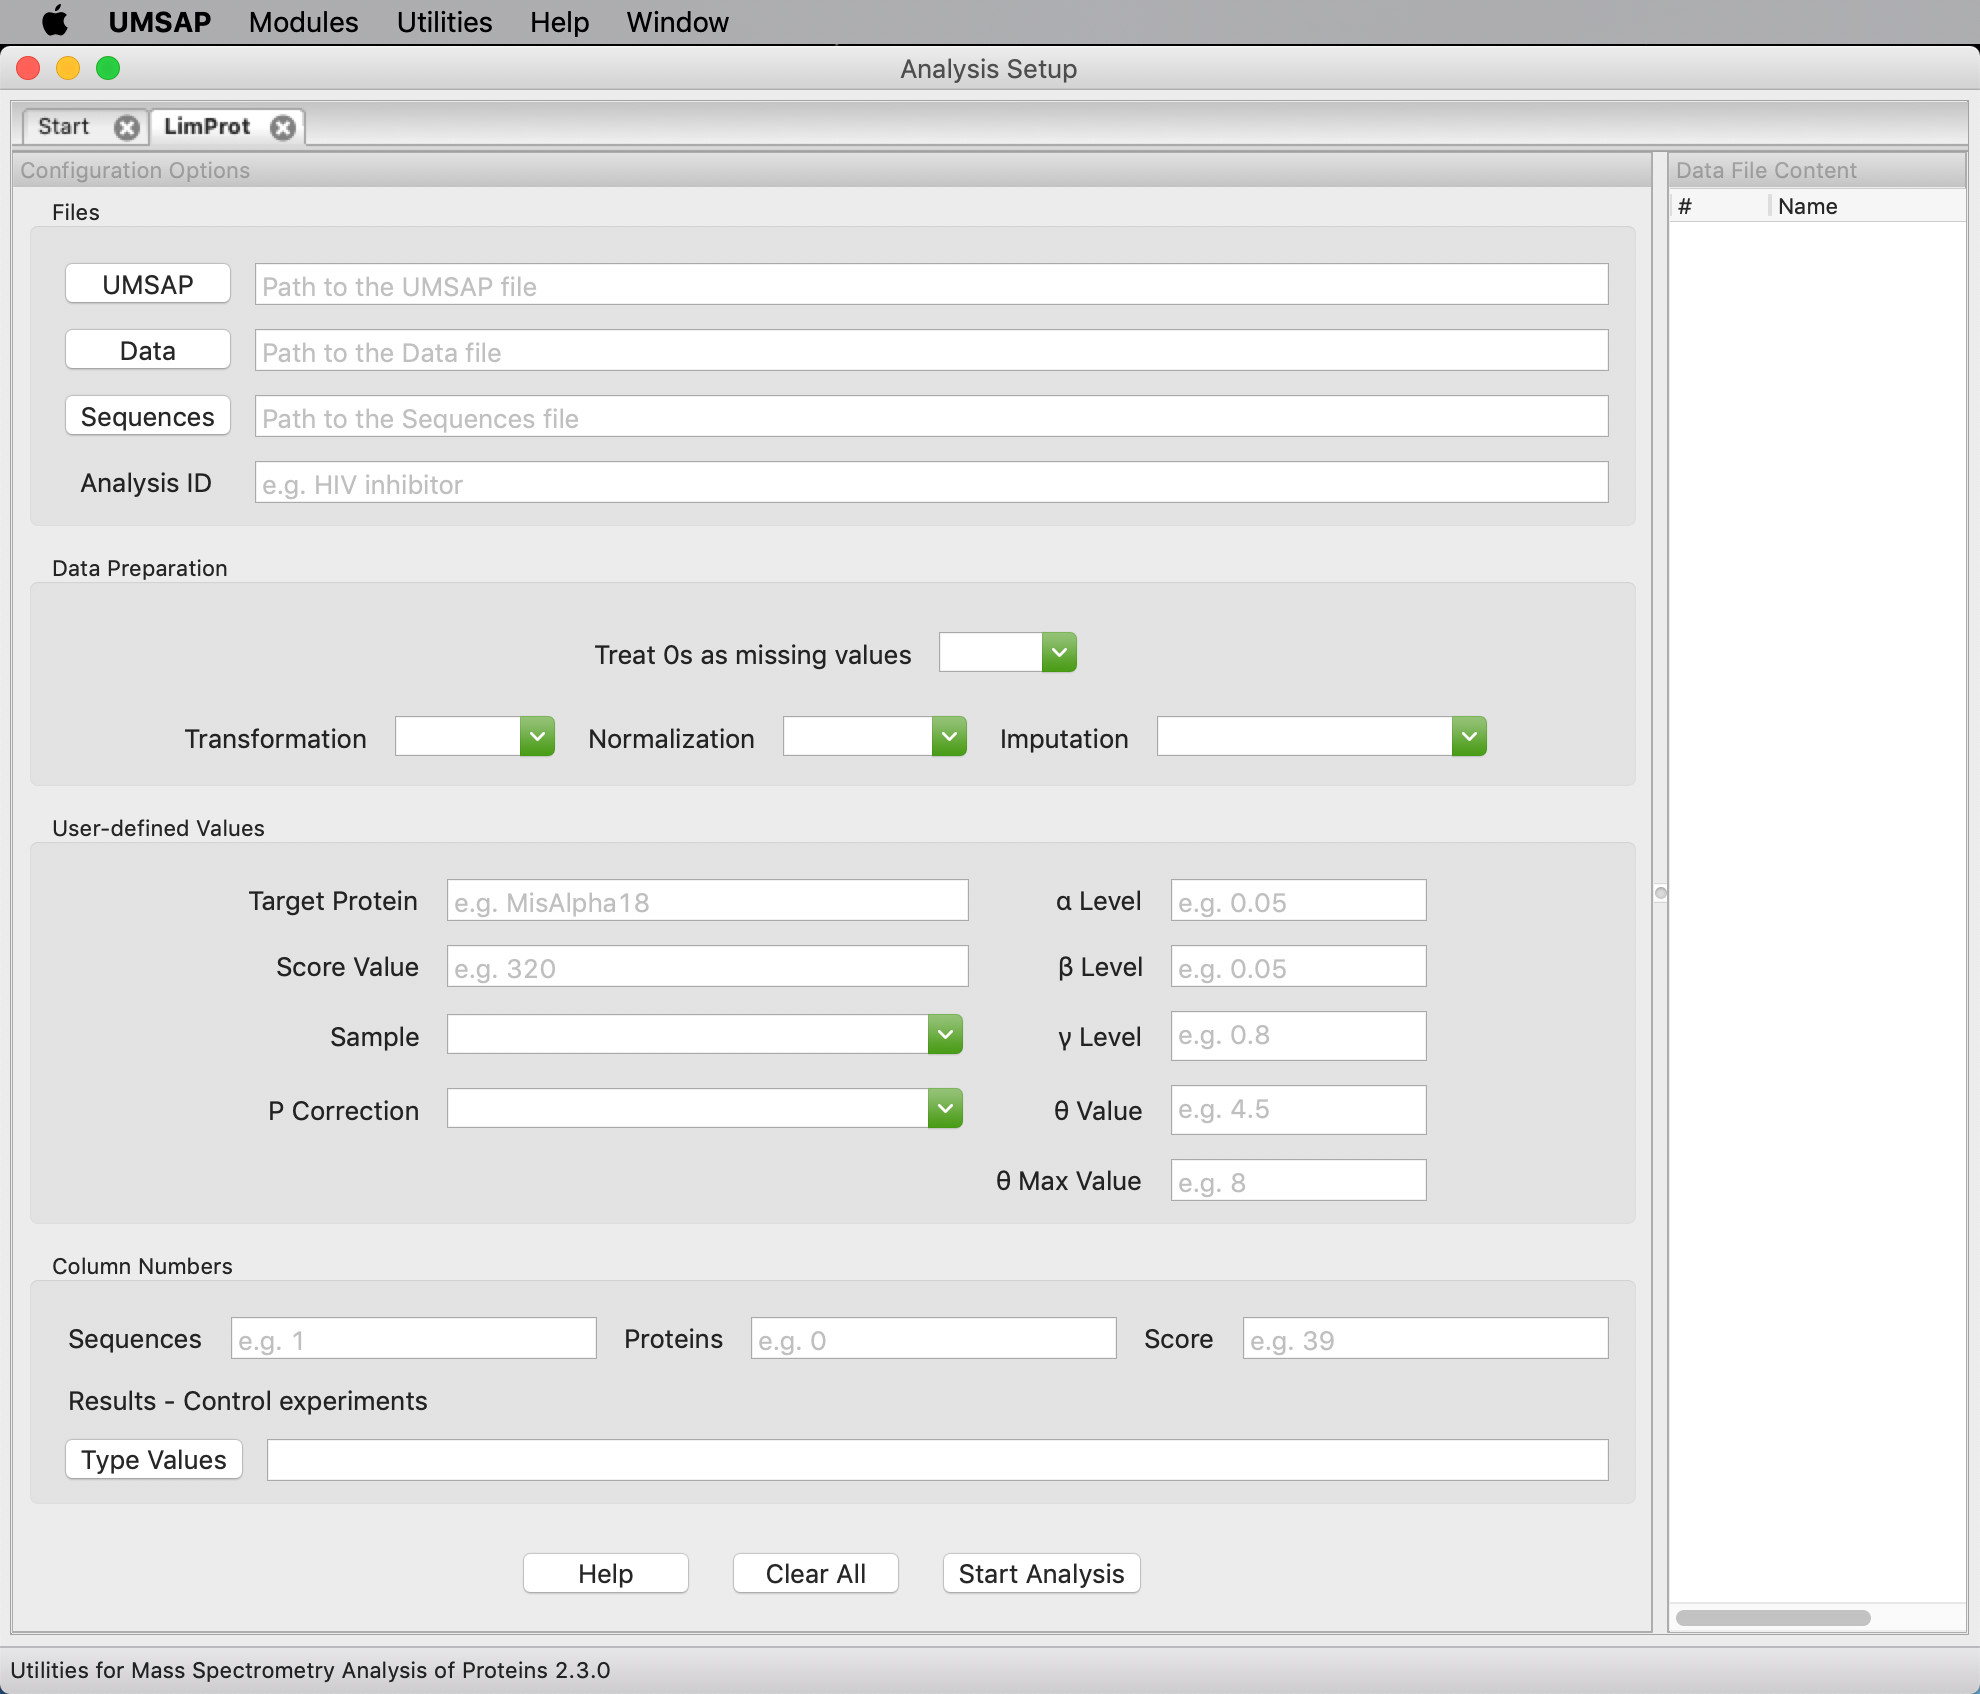
\includegraphics[width=0.7\textwidth]{./IMAGES/MOD-LIMPROT/limprot-mod.jpg}
	\caption[The Limited Proteolysis module window]{\textbf{The Limited Proteolysis module window.} This window allows users to performed the analysis of the results obtained during a two steps enzymatic proteolysis experiment where the products from the first limited digestions are separated using SDS-PAGE electrophoresis. Optional parameters default to NA when the window is created. The rest of the parameters must be provided by the user.} 
	\label{fig:limprotMainWindow}
	\vspace{-5pt} 	
\end{figure} 

\num{4}.- The Output folder\label{par:limprotOutFolder} button allows users to browse the file system and select the location of the folder that will contain the output. By default, UMSAP will create a LimProt folder inside the selected Output folder to save all the generated files. If only the name of the output folder is given, the output folder will be created in the same folder containing the Data file. If this field is left empty, then the LimProt folder will be created in the same folder containing the Data file. If the selected output folder already contains a LimProt folder, then the current date and time to the seconds will be added to the name in order to avoid overwriting the files from previous analyses.

\num{5}.- The Output name button does nothing but the text box to its right allows users to specify the name of the files that will be generated during the analysis. If this field is left empty, then the name limprot will be used for the output files. 

The section \textit{Values} of Region \num{2} contains nine parameters. Here, users provide information about the Target protein, how the Data file should be processed and which optional analysis will be performed.

\phantomsection
\num{1}.- The parameter Target protein\label{par:limprotTargetProtein} allows users to specify which of the proteins detected in the MS experiments was used as substrate during the enzymatic digestions. Users may type here any unique protein identifier present in the Data file. The search for the Target protein is case sensitive, meaning that eFeB is not the same as efeb.

\phantomsection
\num{2}.- The parameter Score value\label{par:limprotScoreValue} allows users to define a threshold value above which the detected peptides will be considered as relevant. The Score value is an indicator of how reliable was the detection of the peptide during the MS experiments. The value given to UMSAP depends on the program generating the Data file. Only one real number equal or greater than zero will be accepted as a valid input here. A value of zero means all detected peptides belonging to the Target protein will be treated as relevant peptides.

\num{3}.- The parameter Data normalization allows selecting the normalization procedure to be performed before running the analysis of the data in the Data file. Currently, only a $\log_2$ normalization is possible but this will be expanded to include quantile, variance stabilization and local regression normalization, among other methods. 

\phantomsection
\num{4}.- The parameter Sequence length\label{par:limprotSeqL} allows users to define the number of residues per line in the sequence file, see \autoref{subsec:utilSeqAli} for more details. Only one integer number greater than zero will be accepted here. A value of NA means that the sequence file will not be generated.

\numrange[range-phrase = --]{5}{9}.- The parameters $\alpha$, $\beta$, $\gamma$, $\Theta$ and $\Theta$max are used to configure the equivalence test\cite{Limentani2005} performed to identify peptides in the selected gel spots with a similar intensity values to the control spots. See \autoref{sec:limprotEquivalenceTest} for more details.

The section \textit{Column numbers} of Region \num{2} contains five parameters. Here, users provide the column numbers in the Data file from where UMSAP will get the information needed to perform the analysis of the limited proteolysis results. All columns specified in this section must be present in the Data file. Users must be aware that Python starts counting from \num{0}. Therefore, the number of the columns in the Data file starts from \num{0} and not from \num{1}. The column numbers displayed in the list box of Region \num{3} after the Data file is selected can be directly used for the Column numbers values.  

\num{1}.- The parameter Sequences allows users to specify the column in the Data file containing the sequences of the peptides identified in the MS experiments. Only one integer number equal or greater than zero will be accepted here.

\num{2}.- The parameter Detected proteins allows users to specify the column in the Data file containing the unique protein identifier for the proteins detected in the MS experiments. It is in this column where the program will look for the Target protein value given in the section \textit{Values} of Region \num{2} of the interface. It is important that in this column the Target protein value is used to refer to only one protein. Only one integer number equal or greater than zero will be accepted here.

\num{3}.- The parameter Score allows users to specify the column in the Data file containing the Score values. It is in this column where the program will look for the values to be compared against the Score threshold given in the section \textit{Values} of Region \num{2} of the interface.

\phantomsection
\num{4}.- The parameter Columns to extract\label{par:limprotColumnExtract} allows users to specify which columns in the Data file will be copy to the shorter versions of the Data file, see page \pageref{subsec:utilShortDF} for more details. A range of columns may be specified as \numrange[range-phrase = --]{4}{10} with both numbers included in the range. Any number of columns may be specified here. Only integer numbers equal or greater than zero will be accepted. A value of NA means no shorter version of the Data files will be created.

\phantomsection
\num{5}.- \label{par:limprotResultControl}The parameter Results - Control experiments allows users to specify the columns in the Data file containing the results of the control and enzymatic digestion experiments. For the Limited Proteolysis module, there are three ways to provide the information for this parameter. Users can directly type the column numbers corresponding to the control and digestion experiments, load the values from a .txt file using the Load values button or use the Type values button to call a helper window, see \autoref{fig:limprotResControlWindow}. 

Independently of the chosen method, the expected input here is a matrix in which each element contains the column numbers with the MS results for a gel spot. Matrix elements are coma (,) separated while rows are semicolon (;) separated. Notice that the last row does not end with a semicolon (;). The first row of the matrix should contain only one element corresponding to the control experiments. Duplicate column numbers are not allowed. 

The helper window is divided in four Regions. Region \num{1} allows to define the number of bands and lanes of interest in the gel and create the matrix in Region \num{2}. Each text field in Region \num{2} should contain the column numbers with the MS results for the given gel spot. The values for the text fields should be positive integer numbers or a range of integers, e.g. \numrange[range-phrase=--]{60}{62} or NA for empty gel spots. Fields left empty are set to NA when the values are exported to the window of the module. The column numbers can be seen in the list box in Region \num{3}. Selected entries in the list box can be copied and then pasted to the text fields using the right mouse button or the Tools menu. Region \num{4} contains two buttons to Cancel or to Export the values to the window of the module. 

\begin{figure}[h]
	\centering
	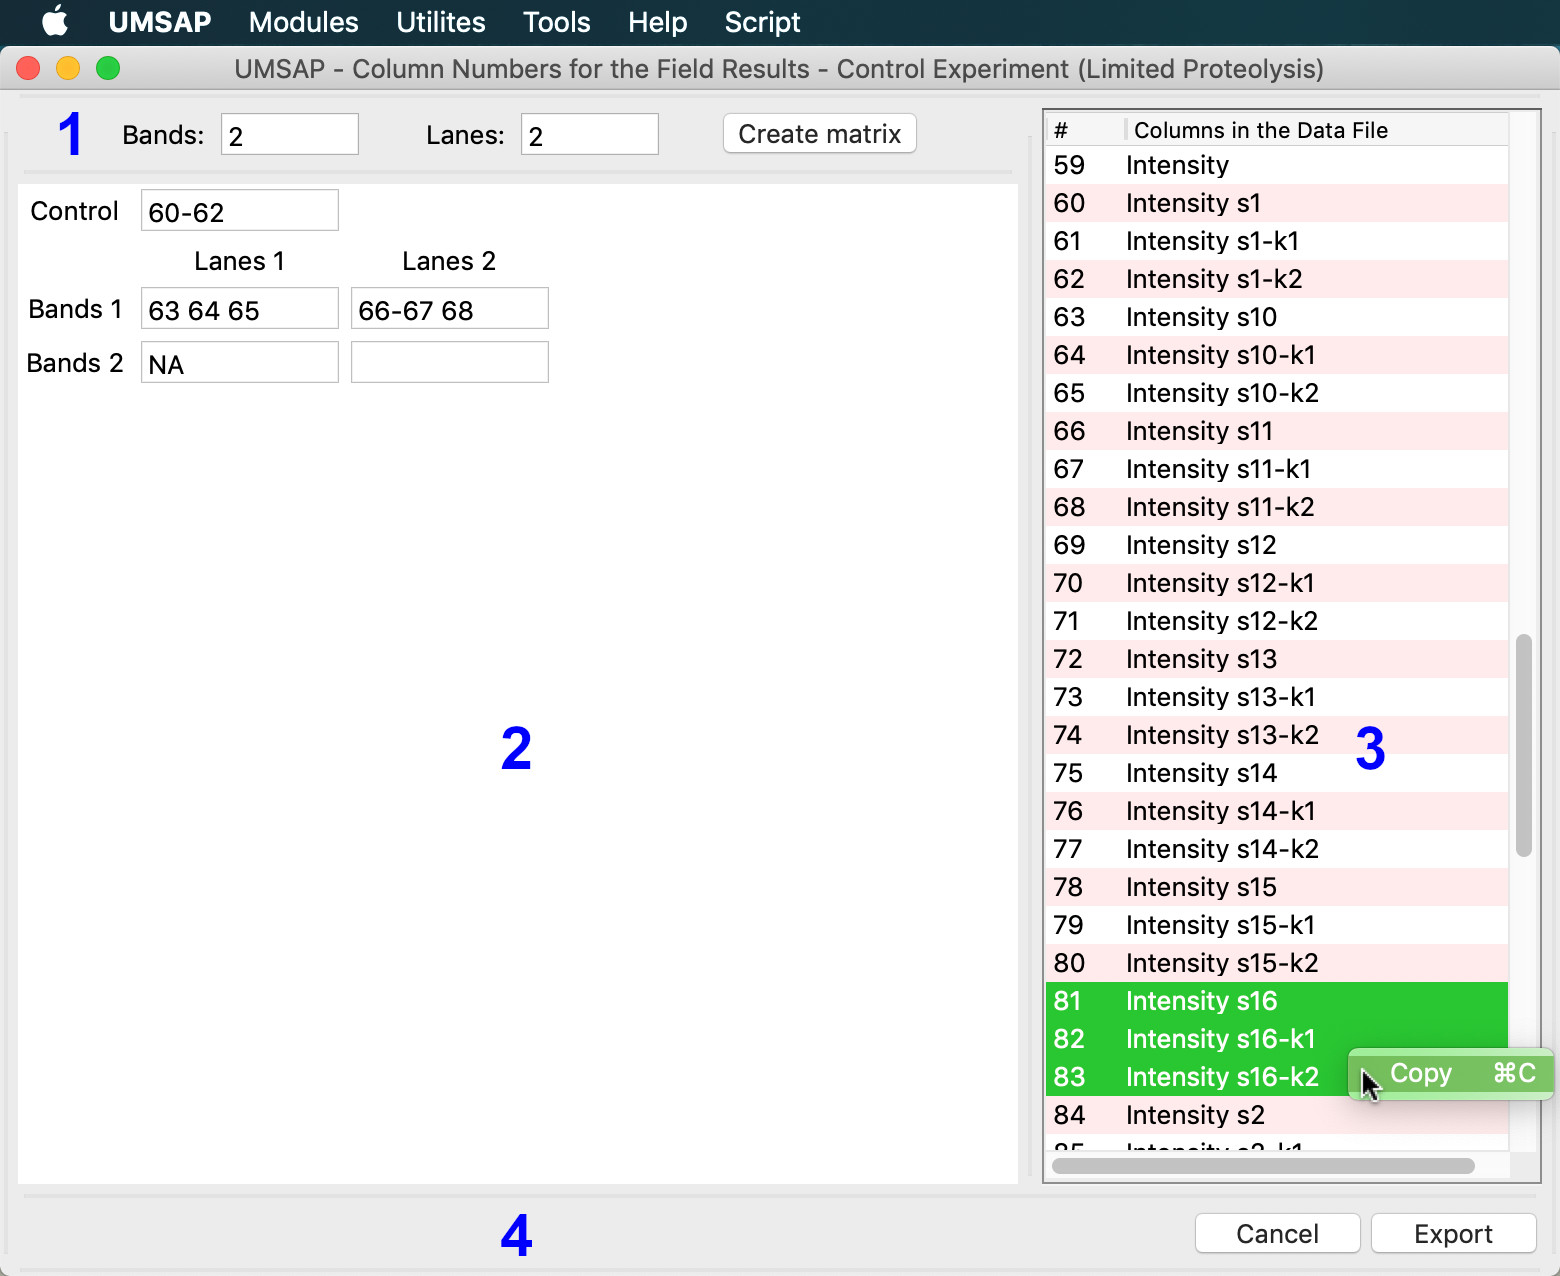
\includegraphics[width=0.7\textwidth]{./IMAGES/MOD-LIMPROT/limprot-rescontrol.jpg}
	\caption[The Result - Control experiments helper window for the Limited Proteolysis module]{\textbf{The Result - Control experiments helper window for the Limited Proteolysis module.} This window allows users to specify the column numbers in the Data file containing the MS results for the selected gel spots.} 
	\label{fig:limprotResControlWindow}
	\vspace{-5pt} 	
\end{figure}

The column numbers can also be loaded from a .txt file. The format of the file content is very simple. Each row of the file will be a row of the matrix and column's content are separated by a comma (,). The first row in the file will be the columns for the control experiment and no commas are needed in this case. The following example will create the same matrix shown in \autoref{fig:limprotResControlWindow} after the .txt file is loaded.

\numrange[range-phrase=--]{60}{62}\newline
\num{63} \num{64} \num{65}, \numrange[range-phrase=--]{66}{67} \num{68}\newline
NA, \numrange[range-phrase=--]{70}{72} 

The same matrix can be directly typed in the text field of the parameter Results - Control experiments of Region \num{2} of the interface of the module. The text to typed is similar to the content of the .txt file discussed in the previous paragraph. The only difference is that semicolons (;) are used to separate rows in the matrix. Text example:

\numrange[range-phrase=--]{60}{62}; \num{63} \num{64} \num{65}, \numrange[range-phrase=--]{66}{67} \num{68}; NA, \numrange[range-phrase=--]{70}{72}

Region \num{3} of the Limited Proteolysis module main window contains a list box that will display the number and name of the columns found in the Data file. The list box is automatically filled when the Data file is selected. Selected columns in the list box can be directly added to any field in the section \textit{Column numbers} of Region \num{2} of the module interface using the right mouse button over the list box or the Tools menu.

Region \num{4} contains two buttons and the progress bar. The Help button leads to an online tutorial while the Start analysis button will trigger the processing of the data file. The progress bar will give users a rough idea of the remaining processing time, once the analysis is started.

\subsection{The Tools menu}

The tools menu in the module window allows to copy the selected columns in the list box of Region \num{3} of the interface to the fields of section \textit{Column numbers} of Region \num{2}. The list box of Region \num{3} of the interface can also be cleared. In addition, through this menu users can create a .uscr file with the given options to the module before running the analysis. If something goes wrong during the analysis, having the .uscr file means that users do not have to type the values of all the parameters again, see \autoref{subsec:utilUscrFile} for more details. 

\section{The analysis}
\label{sec:limprotEquivalenceTest}
First, UMSAP will check the validity of the user provided input. Then, the Data file is processed as follow. All rows in the Data file containing peptides that do not belong to the Target protein are removed. Then, all rows containing peptides from the Target protein but with Score values lower than the user defined Score threshold are removed. These steps leave only relevant peptides, this means, peptides with a Score value higher than the user defined threshold that belong to the Target protein. For each one of these relevant peptides the equivalence test is performed \cite{Limentani2005}.

The implementation of the equivalence test is based on the following equations:
\begin{equation}
	\label{eq:limprotDeviationUpperLimit}
	s^* = s\sqrt{\frac{n-1}{\chi^2_{(\gamma, n-1)}}}
\end{equation}
\begin{equation}
\label{eq:limprotAcceptanceCriterion}
\Theta = \delta + s^*\left[t_{(1-\alpha, 2n-2)} + t_{(1-\beta/2, 2n-2)}\right]\sqrt{\frac{2}{n}}
\end{equation}
\begin{equation}
\label{eq:limprotEquivalenceTest}
(\bar{y}_1 - \bar{y}_2) \pm t_{(1-\alpha, n_1+n_2-2)} \cdot \sqrt{s^2_p\left(\frac{1}{n_1}+\frac{1}{n_2}\right)}
\end{equation}

where $s^*$ is an estimate of the upper confidence limit of the standard deviation, $\chi^2_{(\gamma, n-1)}$ is the ($100\gamma$)th percentile of the chi-squared distribution with $n-1$ degrees of freedom, $\Theta$ is the acceptance criterion, $\delta$ is the absolute value of the true difference between the group's mean values, $t$ is the Student's $t$ value, $\bar{y}$ is the measurement mean and $s_p$ is the pooled standard deviation of the measurements calculated with:
\begin{equation}
\label{eq:poolStDev}
s_p =  \sqrt{\frac{(n_1-1)s^2_1+(n_2-1)s^2_2}{n_1+n_2-2}}
\end{equation}
$\alpha$, $\beta$, $\gamma$ and $\Theta$ are the parameters defined in section Values of Region \num{2} of the main window of the module.

In essence, for each relevant peptide, the control experiments are used to estimate the upper confidence limit for the standard deviation using \autoref{eq:limprotDeviationUpperLimit} and then the acceptance criterion is calculated with \autoref{eq:limprotAcceptanceCriterion}. Finally, the confidence interval for the mean difference for the gel spot and the control is calculated with \autoref{eq:limprotEquivalenceTest} and compare to $\Theta$. Peptides with equivalent mean intensity in at least one gel spot and the control are retained while not equivalent peptides are discarded. 

If the value of $\Theta$ is given in Region \num{2} of the module's interface then only the confidence interval for the mean difference is calculated and the value is directly compared to the given $\Theta$ value. The maximum possible $\Theta$ value must always be provided. The reason for this is that when only a few replicates of the experiments are performed the calculated $\Theta$ value may be to large and then the equivalence test is not able to detect the peptides with intensity values in the experiments lower than in the control.

If the sequence of the native protein is given the module performs a sequence alignment between the native and recombinant sequences. The alignment allows UMSAP to translate the results obtained with the residue numbers of the recombinant protein to the residue numbers of the native protein. This is done to facilitate future comparison of results between different recombinant proteins of the same native protein. However, when analyzing the results of the alignment the module assumes that the recombinant and native sequences differs only in the N and C-terminal tags while the sequence between the tags is identical. If this is not the case, e.g. there are point mutations or insertion/deletion in the sequence of the recombinant protein no native sequence file should be given to UMSAP.

After the filtered peptide (FP) are identified the modules creates the output files.

\section{The output files}

All the output generated by the Limited Proteolysis module will be contained in a LimProt folder created inside the selected Output folder. If the Output folder field in section \textit{Files} of Region \num{2} of the interface is left empty, then the LimProt folder will be created in the directory containing the Data file. If the selected Output folder already contains a LimProt folder, then the current date and time to the second will be added to the name in order to avoid overwriting files from previous analyses. By default the LimProt folder will contain two files with extensions .limprot and .uscr and a Data{\_}Steps folder. The name of these files is provided with the Output name field in section \textit{Files} of Region \num{2} of the interface. Depending on the user provided input extra folders and files will be created inside the LimProt folder (\autoref{fig:limprotOutFolder}). For the rest of this chapter we will assume that the user provided name for the Output folder was \textit{t}, the Output name was myLimTest, the Target protein was \textit{Mis18alpha} and all optional analyses were performed.

Information regarding the content and use of the .uscr file can be found in \autoref{subsec:utilUscrFile}.

If the parameter Sequence length is different than NA, then the file myLimTest.seq.pdf will be created. The file contains the sequence of the Target protein with the sequence of the FP highlighted. More details are given in \autoref{subsec:utilSeqHigh}.

If the parameter Columns to extract is different than NA, then the folder Data will be created. The folder will contain several files that are shorter versions of the Data file. These files will contain only information regarding the Target protein. More details are given in \autoref{subsec:utilShortDF}.

The folder Data\_Steps contains a step by step account of all the calculations performed so users can check the accuracy of the calculation or perform further analysis. The files inside Data\_Steps are plain text file with tab separated columns. The first line contains the name of the columns in the file.

A file containing a list of FP can also be generated as indicated in \autoref{subsec:utilExpData}.

\begin{figure}[h]
	\centering
	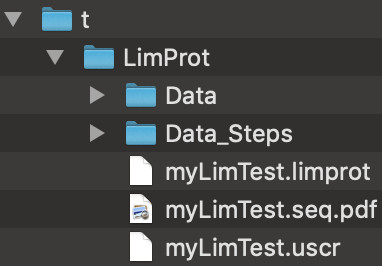
\includegraphics[width=0.35\textwidth]{./IMAGES/MOD-LIMPROT/limprot-files.jpg}	    
	\caption[The structure of the Output folder from the Limited Proteolysis module]{\textbf{The structure of the Output folder from the Limited Proteolysis module.} The folder Data and the file myLimTest.seq.pdf will be created only if requested.} 
	\label{fig:limprotOutFolder}
	\vspace{-5pt} 	
\end{figure}

\section{Visualizing the output files}

The main output of the module is the .limprot file. This file contains the list of FP,  all parameters values and all the information needed to visualize the results with UMSAP. After creating the file at the end of the analysis, the Limited Proteolysis module will automatically load the file and create a windows to display the results, see \autoref{fig:limprotResultsWindow}.

\begin{figure}[h]
	\centering
	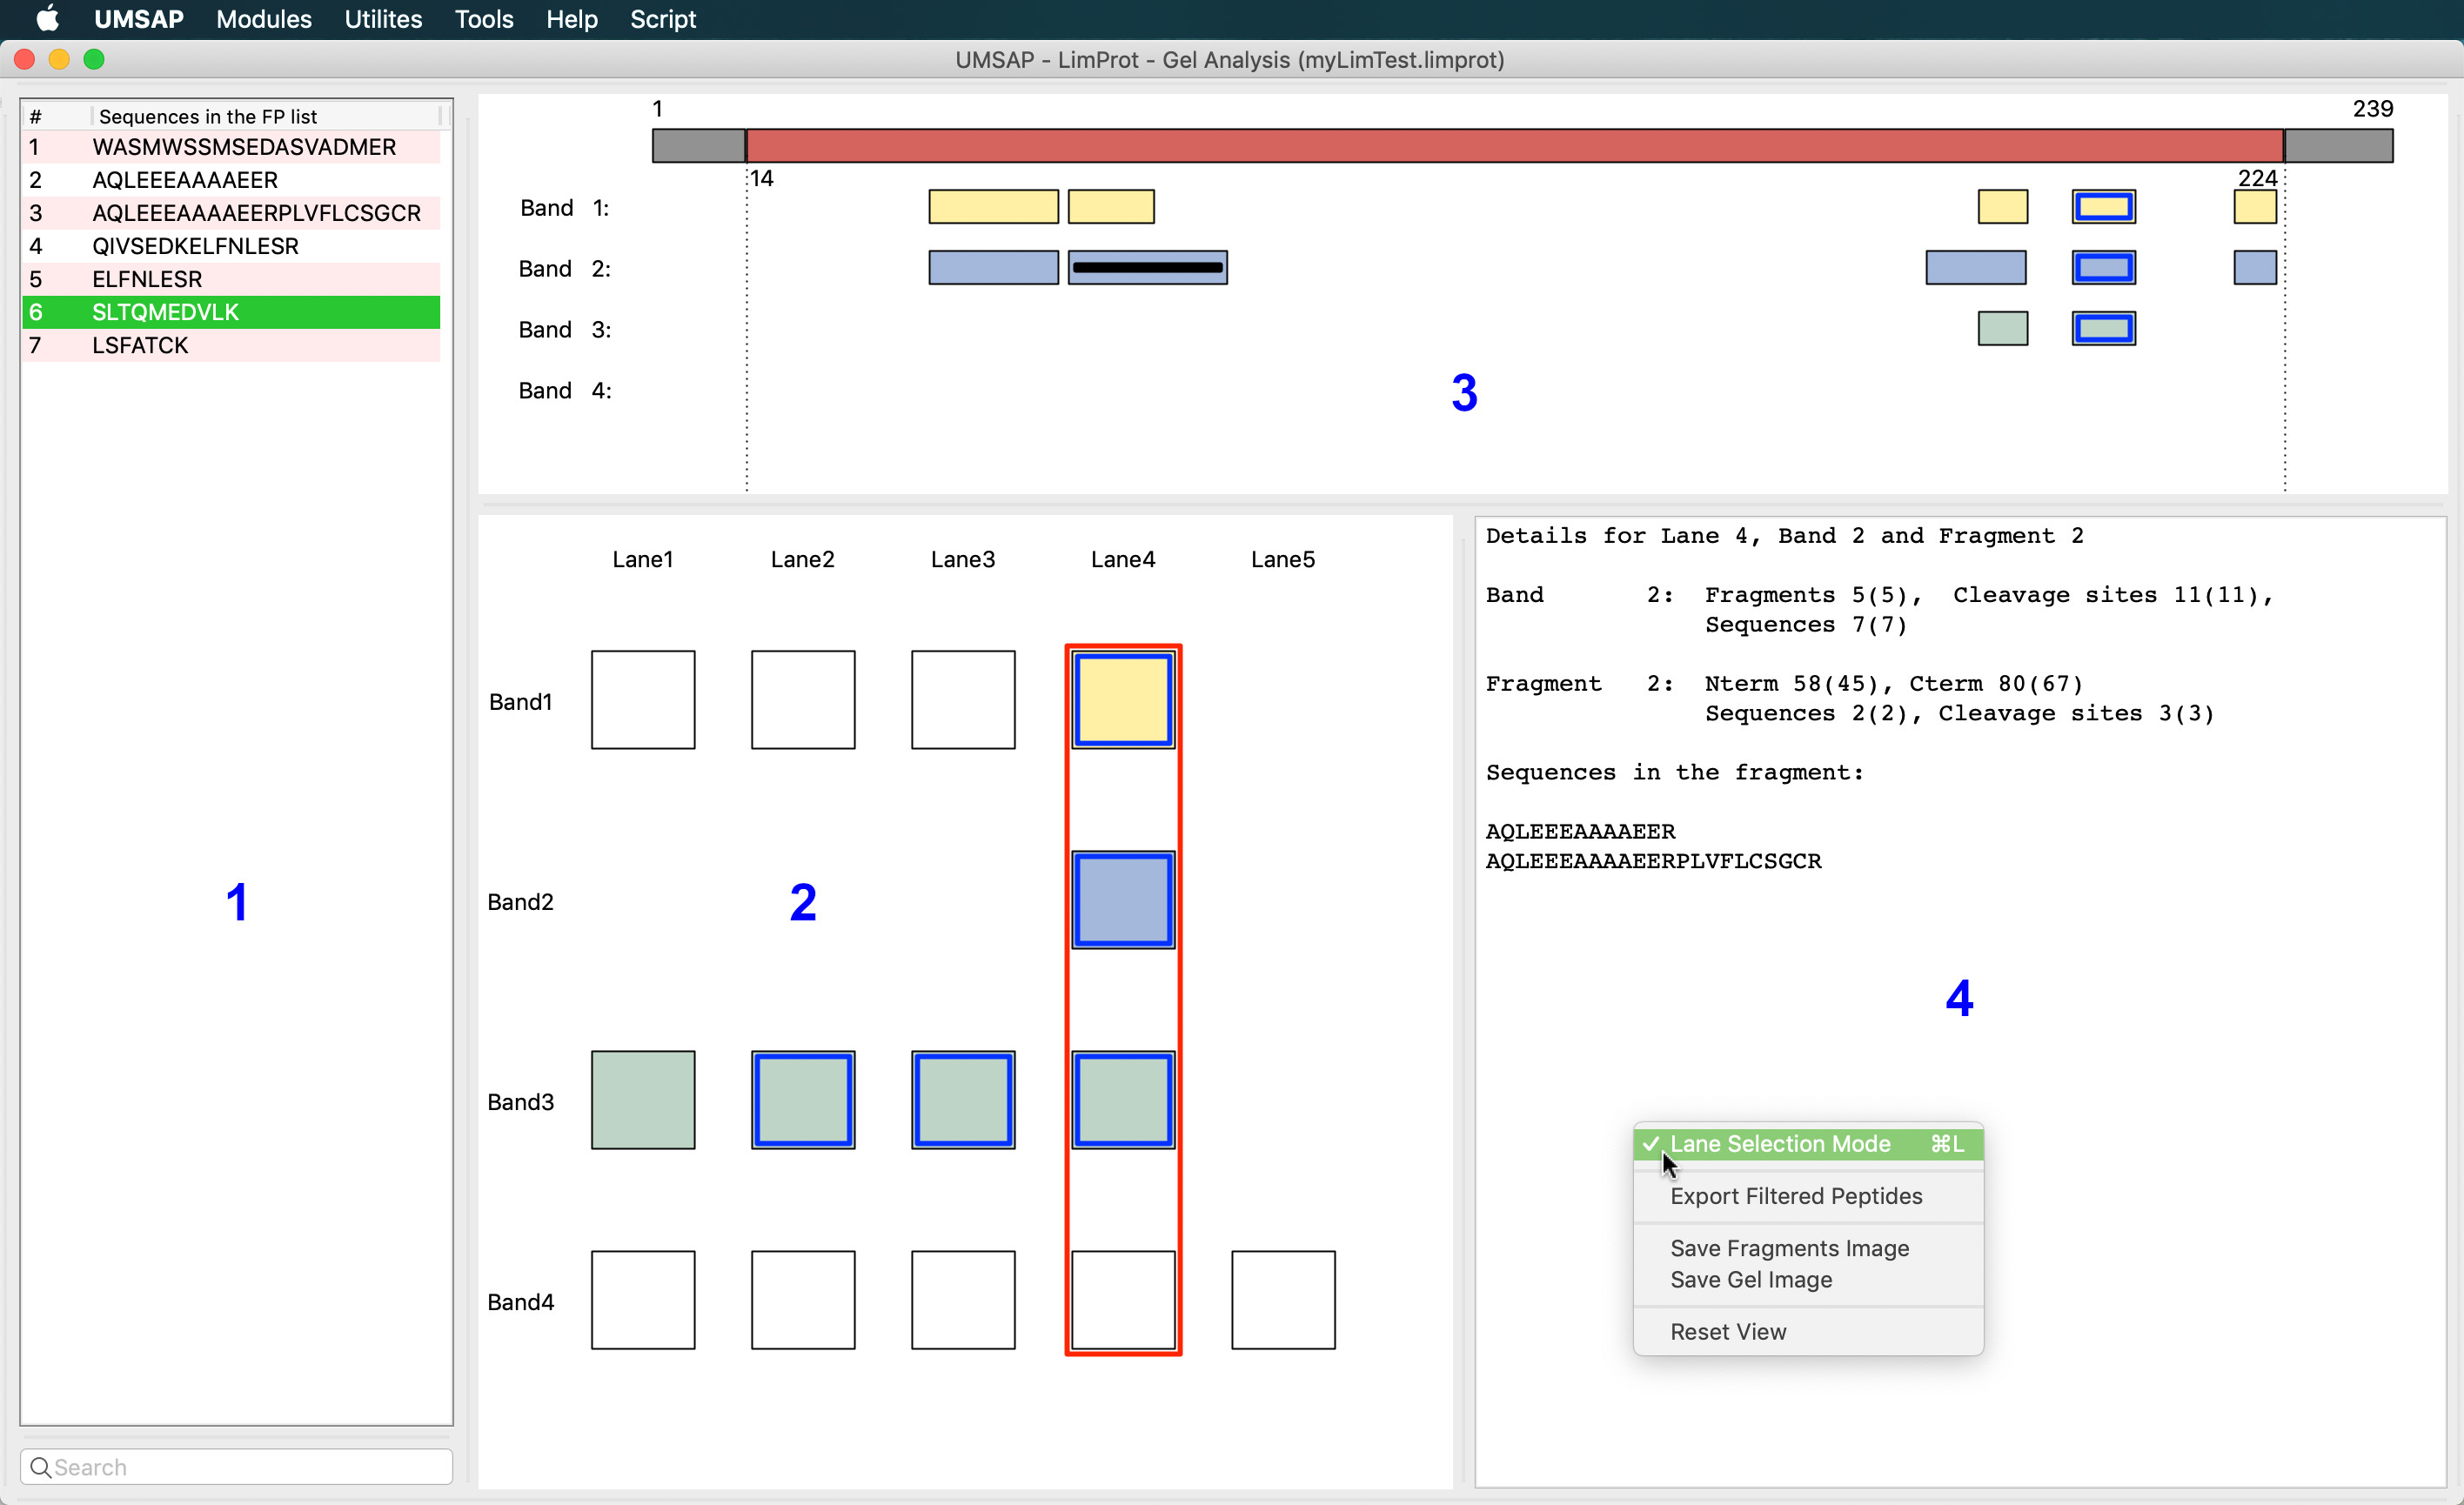
\includegraphics[width=0.8\textwidth]{./IMAGES/MOD-LIMPROT/limprot-frag.jpg}	    
	\caption[The Gel Analysis window]{\textbf{The Gel Analysis window.} Users can performed here the analysis of the fragments obtained in the limited proteolysis experiments.} 
	\label{fig:limprotResultsWindow}
	\vspace{-5pt} 	
\end{figure}

The Gel analysis window is divided in four Regions.

Region \num{1} contains a list of all FP contained in the .limprot file being shown. The search box at the bottom allows to search for a sequence in the list of FP. 

Region \num{2} contains a representation of the analyzed gel. Here, each gel spot is represented with square. When a square is not shown this means that the corresponding gel spot was not analyzed. Empty squares represent gel spot where no peptide from the Target protein was detected with intensity values equivalent to the controls. The rest of the square will be colored according to the band they belong to or the lane. There are two selection modes available for Region \num{2}. In the Lane selection mode selecting one of the Gel spot will also select the entire lane containing the selected gel spot. In this mode the gel spot will be colored according to the band they belong to. The selected lane will be highlighted with a red rectangle. The right mouse button, the Tools menu or the keyboard shortcut Ctrl/Cmd+L can be used to change the selection mode. In the Band selection mode, selecting a gel spot will highlight the band containing the gel spot and the gel spots are colored by lane. Selecting a band or a lane in Region \num{2} will display information about the band/lane in Regions \num{3} and \num{4}.

Region \num{3} will display a graphical representation of the fragments found in each gel spot for the selected band or lane. The first fragment in this region represent the full length of the recombinant sequence of the Target protein. Here, the central red section represents the sequence in the recombinant protein that is identical to the native protein sequence while gray sections represent the sequences in the recombinant protein that are different to the native protein sequence.  If the sequence of the native protein was not given then the fragment is shown in gray. The fragments are color coded using the same colors of the band/lane they belong to.

Selecting a peptide from the list box in Region \num{1} will highlight with a blue border the gel spots in Region \num{2} where the peptide is found. If a lane/band in Region \num{2} is already selected, then the fragments shown in Region \num{3} that contains the selected peptide in the list box will also be highlighted with a blue border.

Region \num{4} will show information about the selected lane/band or gel spot in Region \num{2} or the selected fragment in Region \num{3}. The displayed information for a selected band/lane includes the number of non-empty lanes/bands, the number of fragments identified in each non-empty gel spot in the band/lane and the protein regions identified. Selecting a gel spot will display this information only for the gel spot. Selecting a fragment in Region \num{3} will display in Region \num{4} the following information: number of cleavage sites and fragments, first and last residue number for the selected fragment and a sequence alignment of all peptides forming the fragment.  

\subsection{The Tools menu}
\label{subsec:limprotToolsMenu}

The Tools menu for the window allows changing the selection mode in Region \num{2}, export the data shown in the window (see \autoref{subsec:utilExpData}), save an image of Region \num{2} or \num{3} and to reset the view of the window.

The file containing the exported list of FP will have a tabular format with tab delimited columns. Each row of the file will contain a FP. The columns in the file contain information about the N and C residue numbers, the sequence and Score of the FP. In addition, the results of the equivalence test for each gel spot is given as 0 or 1 value, with 0 meaning not equivalent. The file will have a .txt extension and can be viewed with a simple text editor or Excel.